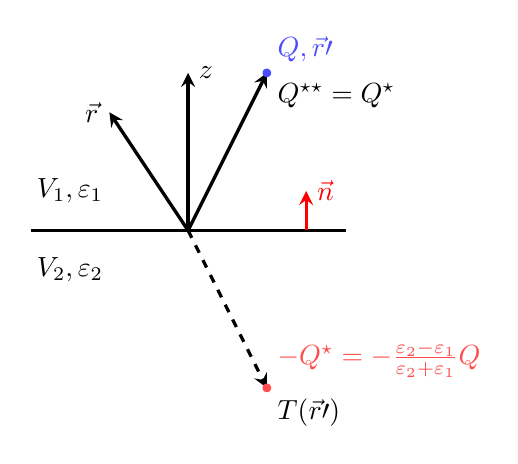
\begin{tikzpicture}[line width = 1.2pt, line join=round,>=stealth]
	\coordinate (O) at (0,0);
	\coordinate (a) at (-2,0);
	\coordinate (b) at (2,0);
	\draw (a) -- (b);
	\draw[color=red, -stealth] (1.5,0) -- (1.5,.5) node[right] {$\vec{n}$};
	\draw[ -stealth] (O) -- (0,2) node[right] {$z$};
	\draw[ -stealth] (O) -- (-1,1.5) node[left] {$\vec{r} $};
	\draw[ -stealth] (O) -- (1,2) node[below right] {$Q^{\star\star}=Q^\star$};
	\filldraw [color=blue!70] (1,2) circle (1pt) node[above right] {$Q, \vec{r}\prime $};
	\draw[ dashed, -stealth] (O) -- (1,-2) node[below right] {$T(\vec{r}\prime )$};
	\filldraw [color=red!70] (1,-2) circle (1pt) node[above right] {$-Q^\star=-\frac{\varepsilon_2-\varepsilon_1}{\varepsilon_2+\varepsilon_1} Q$};
	\draw(-1.5,0.5) node {$V_1,\varepsilon_1$};
	\draw(-1.5,-0.5) node {$V_2,\varepsilon_2$};

\end{tikzpicture}